\graphicspath{{data/SimModule/ElectronicsSimualtion/}}

\chapter[Electronics Simulation]
{Electronics Simulation}
\section{Usage}
\texttt{JPSim} runs Electronics Simulation default. Electronics Simulation can be shut down using parameters \texttt{-e ElectronicsSwitch}.
\begin{lstlisting}[language=bash]
$ JPSim [-e (OFF/ON)] [-dn nDarkNoise[0/1/2/n]]
\end{lstlisting}
\begin{itemize}
    \item {\tt ElectronicsSwitch} or \texttt{-e} and this parameter needs be set mandatory.
    \item {\tt nDarkNoise} default is 1(defined in JPSimTrigger.cc). PreTriggerNoDarkNoise,PreTrigger, PreTriggerFullDarkNoiseFast, PreTriggerFullDarkNoise
    \item 
\end{itemize}
\section{ElecModule Code Structure}
Code files of Electronics Simulation is stored in \texttt{\$JASP\_install/Simulation/ElecModule}. The Structure of above directory is shown in Figure~\ref{fig:elecstructure}.
\begin{figure}[htbp]
    \dirtree{%
    .1 ElecModule/.
    .2 include/.
    .3 JPSimDarkNoise.hh.
    .3 JPSimElecTrigSim.hh.
    .3 JPSimElectronics.hh.
    .3 JPSimPMT.hh.
    .3 JPSimPMTManager.hh.
    .3 JPSimPreTrigger.hh.
    .3 JPSimTrigger.hh.
    .3 VDarkNoise.hh.
    .3 VElecTrigSim.hh.
    .3 VElectronics.hh.
    .3 VPreTrigger.hh.
    .3 VTrigger.hh.
    .2 src/.
    .3 JPSimDarkNoise.cc.
    .3 JPSimElectronics.cc.
    .3 JPSimPMT.cc.
    .3 JPSimPMTManager.cc.
    .3 JPSimPreTrigger.cc.
    .3 JPSimTrigger.cc.
    }
    \caption{{\tt ElectronicsSimulation} directory structure}
    \label{fig:elecstructure}
\end{figure}
\subsection{Brief Introduction to important files}
\begin{description}
    \item[JPSimPMT<.hh/.cc>] Class \texttt{JPSimPMT} set and return parameters of PMTs, 
    which will be set when JSAP initialize Detector geometry implemented by code in \texttt{JPSimDetectorConstruction.cc}.
    \texttt{JPSimPMT} contains many parameters, such as the position, electronics property. It use a charge model to describe
    the gain process of electrons. The charge model obey distribution of Poisson.
    % charge model
    \[P(0, \mu)*w*\alpha*e^{-\alpha x}\]
    The noise model is gauss distribution$N(0, rms)$.
    \item[VElecTrigSim.hh] Virtual Class \texttt{VElectrigSim}
    \item[JPSimDarkNoise<.hh/.cc>]  Class \texttt{DarkNoise}
    \item[JPSimElecTrigSim.hh]\label{JPSimElecTrigSim} \texttt{JPSimElecTrigSim.hh} defines template class \texttt{JPSimElecTrigSim} inherited from class \texttt{VElectrigSim}.
    \begin{lstlisting}[language=C++]
template<class PreTrigger, class DarkNoise,
            class Electronics, class Trigger>
class JPSimElecTrigSim : public VElecTrigSim
    \end{lstlisting}
    Class \texttt{JPSimElecTrigSim} is used as the combination of the above four classes and storage the objects of four classes in each event simulation. In code realization, class JPSimElecTrigSim
    is construct in construction of event simulation in file \texttt{JPSimEventAction.cc}. 
    \begin{lstlisting}[language=C++]
// JPSimEventAction.cc: JPSimEventAction::JPSimEventAction
ets = new JPSimElecTrigSim<JPSimPreTrigger, JPSimDarkNoise,
    JPSimElectronics, JPSimTrigger>();
    \end{lstlisting}
    \item[JPSimPreTrigger<.hh/.cc>] Class \texttt{JPSimPreTrigger} return \texttt{PreTriggers} using information of global PETime(use the computer time as start of time), not the simulated waveform.
    PreTrigger operation accurates the speed of simulation.
    %segmentBegin and segmentEnd:
    %deltat0+detlat1<0 jisimhit<
    \item[JPSimElectronics<.hh/.cc>] Class \texttt{JPSimElectronics} generates waveform according to the parameters of pmt, including charge model, basline noise, DC offset and single photon response(SPE).
    After generate above waveform, \texttt{JPSimElectronics} simulate the process of ADC which change the volatage to ADC address.
    
    \item[JPSimTrigger<.hh/.cc>] Class \texttt{JPSimTrigger} gives formal triggers used to extract readout waveforms.
    \texttt{JPSimTrigger<.hh/.cc>} simulates the process of pulse amplitude discriminator to get logic signal. 
    When the waveform(negative signal) less than the threshold, generate a rectangle logic signal with
    a time width of CoincidenceWindow(default value is 50ns). If the sum of logic signal exceeds nTriggerCondition, a trigger will be
    recorded. After all the triggers generated, readout and triggerinfo will be output.
\end{description}

\subsection{related Classes or code files}
\begin{description}
    \item[G4Module/src/JPSimEventAction.cc] Class \texttt{JPSimEventAction} defines the start of Electronics Simulation, PreTrigger in function \texttt{EndOfEventAction}.
    This class is the entrance of the electronics simlation. The initialization, processing and storage of Electronics Simulation are all done in this part.

    In above section~\ref{JPSimElecTrigSim}, the initialization code of \texttt{JPSimElecTrigSim} is illustrated. The entrance of Electronics Simulation is implement in function \texttt{JPSimEventAction::EndOfEventAction}.
    This function save TruthInfo first, which is the result of detector simulation. After the storage process of TruthInfo finished, Electronics Simulation starts and save TriggerInfo.
    \begin{lstlisting}[language=C++]
// JPSimEventAction.cc:L394
ets->GetPreTriggerPtr()->PreTriggerNoDarkNoise(
    JPSimPMTManager::GetInstance()->HitListMap, 
    JPSimPMTManager::GetInstance()->TempHitBuffer, 
    hitListIntvl, nEventNo);
    \end{lstlisting}
    \texttt{JPSimEventAction} also control the whole process of Electronic Simulation, include PreTrigger, Electronics, Trigger.
    
    \begin{lstlisting}[language=C++]
// JPSimEventAction.cc:L422
ets->GetElectronicsPtr()->Shape(hitItem.first, 
        hitItem.second, WaveformList, HitListMap);
// JPSimEventAction.cc:L428
ets->GetTriggerPtr()->Trigger(hitItem.first, HitListMap, 
        WaveformList, TriggerInfoList, fTrackContainer, 
        TrackMap, fTruthList);
    \end{lstlisting}
    \item[G4Module/src/JPSimTrackingAction.cc] Class \texttt{JPSimTrackingAction} simulates the transportation of electrons in PMT.
    It get the time of each photon hit on the Cathode(HitTime). Then it add the TTS according to different PMTs.
    \item[DataIOModule/src/JPSimDataOutput.cc] This file defined the format of output tree, such as readout and triggerinfo.
    \item[DataIOModule/src/JPSimGDMLReader.cc] Class \texttt{JPSimGDMLReader} is called by Class \texttt{JPSimPMT}, and return property
    of PMT read from GDML files.
    \item[DetectorStructure/] Storage detector structure, include PMT positon and type.
    \item[PMTCalib/] Storage the property of different types of PMT.
\end{description}
\section{Data Flow}
\subsection{PMT property}
As Figure~\ref{ElecSimDataFlow} illustrated in the left part, GDML files are read by GDML Reader. It parse GDML into different value and set properties of PMT, 
such as TTS, Gain, BaselineRMS and so on.
\begin{lstlisting}[language=c++]
// JPSimGDMLReader.cc:L271
pmt->SetModelName(modelname);

// other parameters also be set
// ...
\end{lstlisting}
GDML Reader also set electronic parameters, such as Trigger threshold, coincidence time, the DCoffset of sample board and so on, in \texttt{JPSimDetectorConstruction}.
\begin{lstlisting}[language=c++]
// JPSimDetectorConstruction.cc:L169
JPSimTrigger::fCoincidenceWindow = fParser->GetConstant(
                                    "Coincidence_Window")*ns;
JPSimTrigger::fThreshold = fParser->GetConstant("Threshold");
JPSimTrigger::nTriggerCondition = fParser->GetConstant(
                                "Trigger_Condition");
JPSimTrigger::fTimeWindow = fParser->GetConstant("Time_Window")*ns;
JPSimTrigger::fTriggerPosition = fParser->GetConstant(
                            "Trigger_Position")*ns;
JPSimTrigger::fDynamicRange = fParser->GetConstant("ADC_DynamicRange");
JPSimTrigger::nBit = fParser->GetConstant("ADC_Bit");
JPSimTrigger::fDCOffset = fParser->GetConstant("ADC_DCOffset");
JPSimTrigger::nBits = TMath::Power(2, JPSimTrigger::nBit);
JPSimTrigger::nThreshold = (UInt_t)TMath::Abs(
    (JPSimTrigger::fThreshold+
        JPSimTrigger::fDCOffset*1000+1000*JPSimTrigger::fDynamicRange)/
        (JPSimTrigger::fDynamicRange*1000/JPSimTrigger::nBits));
\end{lstlisting}
ALL of above properties will be used by Detector simulation and Electronics Simulaiton.
\begin{figure}[htbp]
    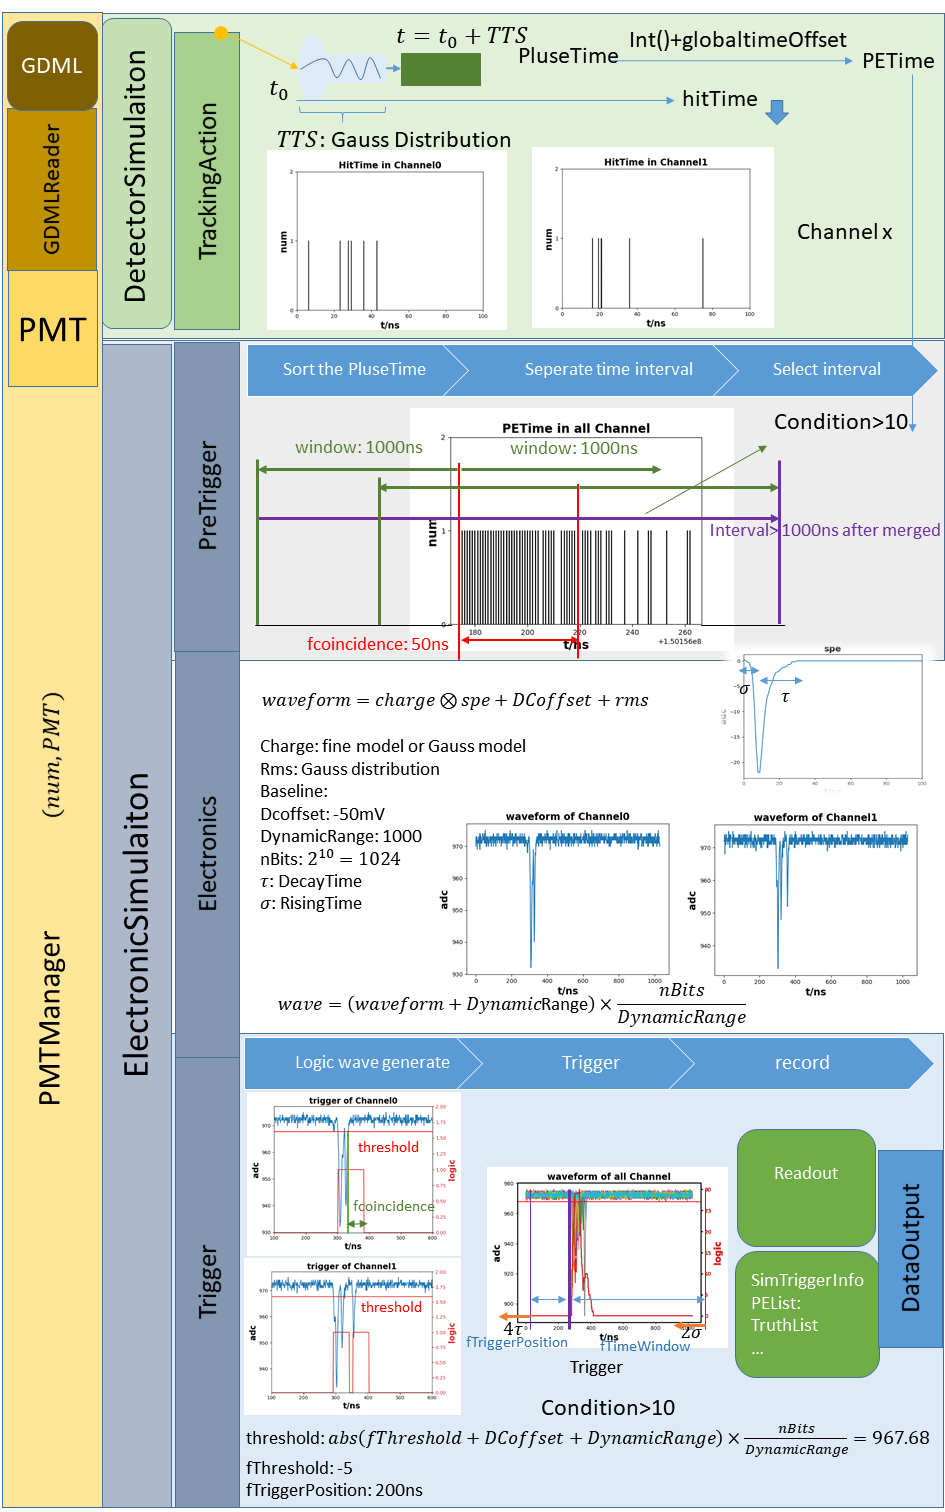
\includegraphics[width=\textwidth]{data/SimModule/ElectronicsSimulation/dataflow.png}
    \label{ElecSimDataFlow}
    \caption{Electronics Simulation Data Flow}
\end{figure}
\subsection{Electronics Simulation in Detector Simulation}
Detector Simulation handle physics process in Detector except PMT. In the head of Figure~\ref{ElecSimDataFlow}, when a track stop at cathode in a PMT,
\texttt{TrackingAction} records the hitTime, $t_0$. The photon will generate electorns and electrons need time(TTS) to fly to the anode. 
\texttt{TrackingAction} use Gauss Distribution to simulate the $TTS$, and add it to $t_0$ as $PluseTime$.
\begin{lstlisting}
    // JPSimTrackingAction.cc:L208
    t += G4RandGauss::shoot(pmt->GetTransitTime(), pmt->GetTransitTimeSpread()/2.355);
\end{lstlisting}
$PluseTime$ is not in line with actual situation because of the sample of \texttt{TDC} is discrete.
The discrete $PETime$ could be get according to the following equation, $globalOffset$ is the global time which is different from Geant4 time:
\[PETime=int(PulseTime)+globalOffset\]
All the information construct to a structure \texttt{hit}, which is returned by \texttt{TrackingAction} and used in \texttt{Pretrigger}.
\subsection{PreTrigger}
Class \texttt{PreTrigger} uses $PETime$ to generate a series of time interval, which is described following:
\begin{description}
    \item[sort $PluseTime$] All hits are sorted by $pulseTime$, because Class \texttt{JPSimHit} overload the $>$ method as following. $t_0$ is $hitTime$ in $ns$,
    while $t_1$ is decimal part in $ns$.
    \begin{lstlisting}
        // DataType/JPSimStruct.hh:L50
        bool operator < (const JPSimHit& rhs) const { 
            double delta0 = this->PETime.t0-rhs.PETime.t0;
            double delta1 = this->PETime.t1-rhs.PETime.t1;
            return delta0+delta1<0; 
        }
    \end{lstlisting}
    \item[seperate and merge time interval] 
    Each $PluseTime$ corresponds with a time interval $[PulseTime-window, PulseTime+window]$, default value of window is $1000ns$.
    After a interval found, the next $PulseTime$ will search since the time of previous $pulseTime$ added $fcoincidence time$, default is $50ns$.
    All of the time intervals merge with others if part of them are overlapped. This step gives some time interval of different 
    length.
    \item[select time interval] check each time intervals and find interval with number of pulse greater than a condition, default is 10.
    Those time intervals will be selected and used by \texttt{Electronics} part.
\end{description}
There are 4 method can be choosed in \texttt{JPSimPreTrigger}. They are different in $DarkNoise$, which are described following:
\begin{enumerate}
    \item \texttt{PreTriggerNoDarkNoise()} Only find the intervals with hits, no dark noise added.
    \item \texttt{PreTrigger()} Only find the intervals with hits, add dark noise and pass them into hitListIntvl
    \item \texttt{PreTriggerFullDarkNoiseFast()} find the intervals with hits, use the dark noise rate to caculate the number of dark noise according to Poisson Distribution.
    \item \texttt{PreTriggerFullDarkNoise()} Generate dark noise of the whole segment to pre-trigger the dark noise accidental trigger. Very slow.
\end{enumerate}
\subsection{Electronics}
\subsubsection{generate volatage waveform}
Class \texttt{JPSimElectronics} is main part in Electronics Simulation and generate the waveform using a series of time intervals.
As the middle of Figure~\ref{ElecSimDataFlow} illustrates, the volatage is caculate as the following equation:
\[waveform=charge\otimes spe+rms+DCoffset\]
The charge model has two option in \texttt{JSAP}.

The $rms$ obeys Gauss distribution, $N(0, rms)$. The $spe$ is gotten from $JPSimPMT$. $DCoffset$ is set by GDML, a property of Electronics board.
\subsubsection{generate ADC waveform}
The volatage waveform will be sampled by ADC. The DCoffset of ADC moves the waveform baseline. The DynamicRange represents the volatage range of ADC, default
is $1000mV$. The default ADC bits is 10, which means $0mV$ maps to $2^10-1=1023$, and $-1000mV$ maps to $0$. This process is described by the following equation:
\[wave=abs(\frac{waveform+DynamicRange}{DynamicRange/2^nBits})\]

\subsection{Trigger}
\subsubsection{generate Trigger}
As illustrated by the bottom of Figure~\ref{ElecSimDataFlow}, class \texttt{JPSimTrigger} use the ADC waveform to generate Trigger, simulate the process of actual 
situation. \texttt{JPSimTrigger} use a threshold, default is 867 and set by different GDML files, to find the time point in each waveform. Once the waveform is smaller 
than the threshold, a logic wave with a length of fcoincidence($50ns$) is generated. Besides, the next search point should begin from 50ns after the previous time point.
After waveform from all PMTs transfer to logic wave, those logic wave are added directly to form a step wave.
A \texttt{Trigger} is generated if the added logic wave is more than a condition, default is 10.
\subsubsection{generate readout and triggerinfo}
Once a \texttt{Trigger} is generated, a time interval, $[Trigger-fTriggerPosition, Trigger+fTimeWindow]$, is extracted to cut a waveform written into \texttt{Readout}.
While the PETruth is more complicated, only PETime during $[Trigger-fTriggerPosition-4\tau, Trigger+fTimeWindow-2\sigma]$ are selected and written into TruthList. $\tau$
is the decay time of SPE while $\sigma$ is rising time of SPE.
\section{Appendix}

This Section ElectronicSimulation is finished by Zhang Aiqiang.

The original figure, root file and programs generating pictures can be found in \url{https://github.com/greatofdream/JSAPElecSimPlot.git}.